%%%%%%%%%%%%%%%%%%%%%%%%%%%%%%%%%%%%%%%%%%%%%%%%%%%%%%%%%%%%%%%%%%%%%%%%%%%%%%%%%%%%%%%%%%%%%%%%%%%%
% ==================================================================================================
% --------------------------------------------------------------------------------------------------
\chapter{Methodology}
In this section we introduce the proposed model and explore its parametrization.
\par
Wherever possible, concepts related to segmentation and classification will be described in their most general sense, since many of the conclusions presented here may also apply to other image analysis and machine learning tasks.
%%%%%%%%%%%%%%%%%%%%%%%%%%%%%%%%%%%%%%%%%%%%%%%%%%%%%%%%%%%%%%%%%%%%%%%%%%%%%%%%%%%%%%%%%%%%%%%%%%%%
\section{Motivation}

Many of the previously proposed WMH segmentation algorithms predict the class of a voxel without any spatial information. In the absence of spatial information, 

The work by \citeauthor{Khademi2012} \cite{Khademi2012,Khademi2014,Khademi2015} was particularly promising, since it overcame many of the usual requirements. These include: the use of multiple MRI modalities, which are not always available; image registration to a common space, which is never perfect and introduces interpolation artifact; the use of training data, which is difficult to find; and assumed Gaussian distribution of tissue graylevels, which is rarely valid.



Assumptions which many models make, and whether they are wrong:

- parametric modelling of graylevel distributions: with single Gaussians: almost certainly wrong. Confounding factors: PVA, parallel MRI signals, motion artifacts, 

The most recent implementation of the EM-fit mixture model by \citeauthor{Ashburner2005} in \cite{Ashburner2005} permits a user-specified number of Gaussian distributions for each tissue class, 

(though convergence is likely challenging)

as well as 

However, the central assumption of these methods is that the distributions of WMH graylevels do not overlap significantly with distributions of any other tissue class.

However, it has been suggested that there is regional heterogeneity in relaxation rates of brain tissues \cite{Sled2004}, and that WMH intensity depends in part on location \cite{Stevenson2000}.

%%%%%%%%%%%%%%%%%%%%%%%%%%%%%%%%%%%%%%%%%%%%%%%%%%%%%%%%%%%%%%%%%%%%%%%%%%%%%%%%%%%%%%%%%%%%%%%%%%%%
\section{Proposed Model}
We now present the proposed model...
\par
The probability of the lesion class $c=1$ in one location $x$, given the features $\by = [y^1,\dots,y^\K]^T$  is modelled as a logistic function parameterized by a vector $\bb = [\b^1,\dots,\b^\K]^T$,
\begin{equation}
  P(c=1\mid\by,\bb) = \frac{1}{1+e^{-\bb^T\by}}
  \label{eq:model}
\end{equation}
This probability -- the estimated lesion label -- is denoted $\hat{c} = P(c=1\mid\by,\bb) \in [0,1]$.
\par
The assumptions of this model include the following:
\begin{itemize}[itemsep=0pt]
  \item only 2 tissues classes are modelled: WMH and healthy brain tissue;
  \item image graylevel(s) and spatial location are sufficient features to discriminate the two classes;
  \item in each voxel, the WMH class is monotonically separable from the healthy class by graylevel(s)
\end{itemize}
% ==================================================================================================
\subsection{Model Fitting}
Fitting the model involves estimating $\bb$ for each voxel $x$. This requires some training data: feature vectors from a population of $N$ observations $\bY = \{\by_1,\dots,\by_\N\}$, and the corresponding labels $\C = \{c_1,\dots,c_\N\}$. The optimal $\bb$ should maximize the likelihood of the model, given this data -- i.e. maximum likelihood estimation (MLE). If the training data are assumed to be independently observed, then the likelihood (conditioned on the data) is defined from binomial theory as 
\begin{align}
  L(\bb\mid\C,\bY) &= \prod_{n=1}^{N} P(c=1\mid\by_n,\bb)^{c_n} \left(1-P(c=1\mid\by_n,\bb)^{1-c_n}\right)\nonumber\\
  &= \prod_{n=1}^{N} \Big[\hat{c}_n^{\en c_n} \left(1-\hat{c}_n^{\en 1-c_n}\right)\Big]
  \label{eq:likelihood}
\end{align}
For computational reasons, it is simpler and asymptotically equivalent to maximize the log-likelihood,
\begin{align}
\L(\bb) &= \log{ \prod_{n=1}^{N} \Big[\hat{c}_n^{\en c_n} \left(1-\hat{c}_n^{\en 1-c_n}\right)\Big] }\nonumber\\
&= \sum_{n=1}^{N} \Big[ c_n \log \hat{c}_n + (1-c_n) \log (1-\hat{c}_n) \Big] \nonumber\\
&= \sum_{n=1}^{N} \Big[ c_n \bb^T\by_n - \log (1+e^{\bb^T\by_n}) \Big] 
\label{eq:loglikelihood}
\end{align}
The optimal $\bb$ is therefore resolved by maximizing the log-likelihood,
\begin{align}
\bb^* &= \underset{\bb}{\arg\max} \en\L(\bb)\nonumber\\
&= \underset{\bb}{\arg\max}\en\sum_{n=1}^{N} \Big[ c_n \bb^T\by_n - \log (1+e^{\et\bb^T\by_n}) \Big]
\label{eq:argmaxmle}
\end{align}
% --------------------------------------------------------------------------------------------------
\subsection{Iterative Updates}
Estimation of $\bb^*$ can be performed using iterative optimization, using an initial estimate $\bb^{(0)}$ and an update term $\Delta\bb^{(t)}$,
\begin{equation}
\bb^{(t+1)} \leftarrow \bb^{(t)} + \alpha\thinspace\Delta\bb^{(t)},
\label{eq:update}
\end{equation}
where $\alpha$ is a small valued learning rate parameter. There are many possible definitions of $\Delta\bb$, including simply the gradient of $\L(\bb)$, denoted $\nabla_{\bb}\L$. However, it can be shown that $\L(\bb)$ is convex, so higher order update equations can be used. The work by \citeauthor{Minka2003} \cite{Minka2003} compares several options, including Newton's method (and variants), conjugate gradient, iterative scaling (and variants), and dual optimization\footnote{Matlab code available at \hreftt{https://github.com/tminka/logreg/}}. For small feature dimensionality ($K$), performance differences among the options were small. Classic Newton updates gave a good balance between memory requirements and computational order, so they are used.
\par
If the gradient $\nabla_{\bb}\L$ and Hessian matrix $\nabla^2_{\bb}\L$ are defined as
\begin{align}
\nabla_{\bb}\L &= \left[\begin{array}{c}
\frac{\d L}{\d\b^1}\\\vdots\\\frac{\d L}{\d\b^\K}
\end{array}\right],\label{eq:llgradient0}\\
\nabla^2_{\bb}\L &= \left[\begin{array}{ccc}
\frac{\d^2 L}{\d\b^1\d\b^1}&\cdots&\frac{\d^2 L}{\d\b^1\d\b^\K}\\
\vdots&\ddots&\vdots\\
\frac{\d^2 L}{\d\b^\K\d\b^1}&\cdots&\frac{\d^2 L}{\d\b^\K\d\b^\K}
\end{array}\right]\label{eq:llhessian0},
\end{align}
then the Newton update is given by
\begin{equation}
\Delta\bb = -{\nabla^2_{\bb}\L}^{-1}\nabla_{\bb}\L.
\label{eq:newtonmle}
\end{equation}
In the current model, the gradient is given by 
\begin{equation}
\nabla_{\bb}\L = \sum_{n=1}^{N} \by_n\left(c_n - \hat{c}_n\right),
\label{eq:llgradient}
\end{equation}
and the Hessian by
\begin{equation}
\nabla^2_{\bb}\L = \sum_{n=1}^{N} \by_n{\by_n}^T \left(c_n - \hat{c}_n\right).
\label{eq:llhessian}
\end{equation}
Substituting (\ref{eq:llgradient}) and (\ref{eq:llhessian}) into (\ref{eq:newtonmle}), the explicit update  $\Delta\bb$ for (\ref{eq:update}) is obtained.
% --------------------------------------------------------------------------------------------------
\subsection{Implementation}

%%%%%%%%%%%%%%%%%%%%%%%%%%%%%%%%%%%%%%%%%%%%%%%%%%%%%%%%%%%%%%%%%%%%%%%%%%%%%%%%%%%%%%%%%%%%%%%%%%%%
\section{Bias Correction \& Registration}



%%%%%%%%%%%%%%%%%%%%%%%%%%%%%%%%%%%%%%%%%%%%%%%%%%%%%%%%%%%%%%%%%%%%%%%%%%%%%%%%%%%%%%%%%%%%%%%%%%%%
\section{Graylevel Standardization}

\clearpage
%%%%%%%%%%%%%%%%%%%%%%%%%%%%%%%%%%%%%%%%%%%%%%%%%%%%%%%%%%%%%%%%%%%%%%%%%%%%%%%%%%%%%%%%%%%%%%%%%%%%
\section{Regularization}
Even if perfect registration and graylevel standardization are achieved, three challenges remain for the VLR model. These challenges involve contradictions between prior knowledge and the MLE-fitted model using the available training data. That is, these challenges could all be overcome by a more complete training set, but this is usually not available. The three challenges are:
\begin{enumerate}
  \item \label{mlech:separable} \textbf{Separable classes:} 
  When data from two classes are perfectly separable, the MLE error surface in parameter space has a convex global minimum at infinity. As a result, the fitted logistic model in voxels with separable data approaches a step-function, since $\b^1\rightarrow+\infty$. This implies that on either side of a specific graylevel threshold ($\tau$), the model is either 100\% confident in predicting the non-lesion class, or 100\% confident in predicting the lesion class. In fact, no threshold is ever so perfect, and instead a level of uncertainty should be maintained around the decision boundary. These two cases are illustrated in Figure \ref{fig:mlech-sep}.
  \item \label{mlech:sparse} \textbf{Sparsely observed lesion class:} 
  Since WML are often distributed in consistent locations, many brain regions contain no lesions across the entire training dataset. In some locations (e.g. the GM), this is expected, while in others (e.g. juxtacortical WM) our prior knowledge predicts lesions will eventually be observed. As illustrated in Figure \ref{fig:mlech-noles}, the MLE-fitted model does not maintain the ability to predict $\hat{c} = 1$ in this location, regardless of the features. However, we would like to keep this ability in many of these locations. 
  \item \label{mlech:noisy} \textbf{Noisy parameter images:} 
  Modelling every voxel independently is risky. We assume that similar locations will contain similar training data, yielding smooth parameter images, which we expect. If this assumption is sometimes invalid, parameter images could contain noise or discontinuities, creating artifacts in estimated lesion class images.
\end{enumerate}
\begin{figure}
  \centering
  \begin{subfigure}{\plotwidth}
    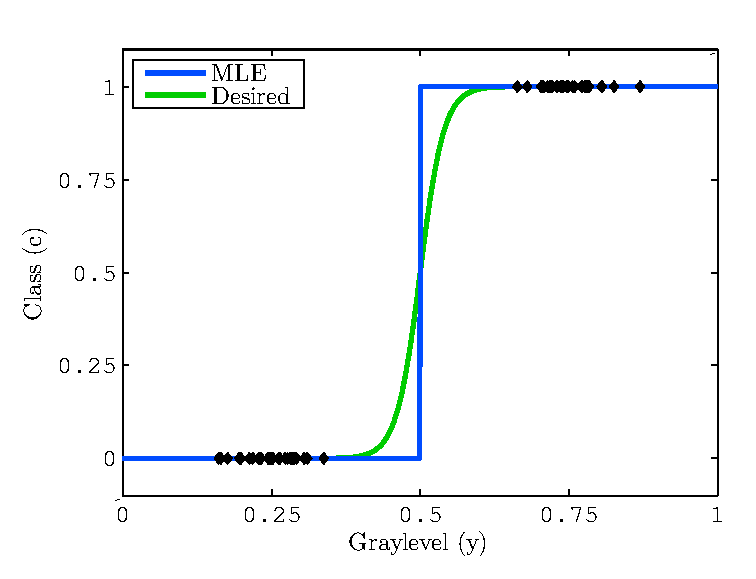
\includegraphics[width=\textwidth]{mlechallenge-sep}\caption{Separable classes}\label{fig:mlech-sep}
  \end{subfigure}
  \begin{subfigure}{\plotwidth}
    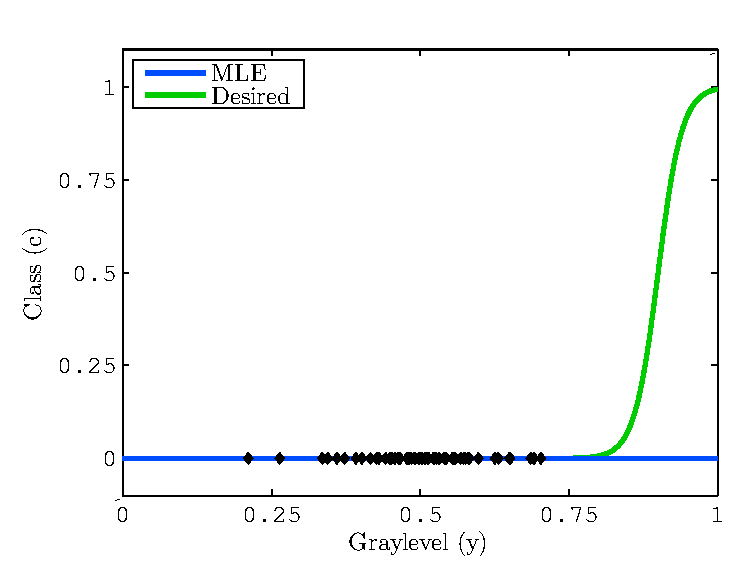
\includegraphics[width=\textwidth]{mlechallenge-noles}\caption{No lesions}\label{fig:mlech-noles}
  \end{subfigure}
  \caption{Challenges encountered using ML estimation of a logistic model.}
  \label{fig:mlech}
\end{figure}
Solutions to these problems are called regularizations -- methods of injecting prior knowledge about the expected model into the optimization. Model fitting which includes regularizations is termed maximum a posteriori (MAP) estimation. Several regularization strategies are explored below.
% ==================================================================================================
\subsection{Data Augmentation}
Noting the central role of training data in each of the above challenges, methods of artificially increasing the training dataset size may be particularly useful in solving them. Data augmentation has long been used in machine learning tasks with limited training data, and there are several methods of generating synthetic data. In low dimensional input/output spaces, random sampling of fitted class-conditional posterior distributions can produce reasonable samples with known labels \cite{Tanner1987}. In higher dimensional problem spaces, however, imputation is more difficult \cite{Goodfellow2014}. For example, the space of potential $100\times100\times100$-sized images has $100^3$ dimensions (one per voxel), yet only a small inner subspace represents plausible images. Generating synthetic examples in this space is therefore challenging, especially for segmentation tasks, where the outputs have dimensionality roughly equal to the input.
\par
Alternatively, simple image manipulations can still afford model improvements \cite{Krizhevsky2012}. In segmentation tasks, both the input image(s) and the corresponding label images can be translated, reflected, rotated, and perhaps resized, thereby avoiding the generation of genuinely synthetic examples. In the current task, 

% ==================================================================================================
\subsection{Classic Regularization}
Challenge \ref{mlech:separable} is well-known in regression problems, and a good solution is to penalize the magnitude of model parameters using the $L_p$-norm: $\lambda\norm{\bb}_p$ \cite{Zou2005}. It can be shown that $L_1$ regularization corresponds to a Laplacian prior on elements of $\bb$, with scale parameter inversely proportional to $\lambda$ (equivalently, this assumes that the model error follows this distribution); similarly, $L_2$ regularization implies a Gaussian prior, with standard deviation inversely proportional to $\lambda$ \cite{Zou2005}. The penalty is appended to the objective function (\ref{eq:argmaxmle}), as in 
\begin{align}
\bb^* &= \J(\bb)\nonumber\\
&= \underset{\bb}{\arg\max}\en\L(\bb) - \lambda\norm{\bb}_p \nonumber\\
&= \underset{\bb}{\arg\max}\en\sum_{n=1}^{N} \Big[ c_n \bb^T\by_n - \log (1+e^{\et\bb^T\by_n}) \Big] - \lambda\norm{\bb}_p
\label{eq:argmaxmap}
\end{align}
Due to its relatively large gradient near zero, $L_1$ regularization is typically used to encourage sparsity in the feature weights (i.e. $\b^k\rightarrow0$) \cite{Tibshirani1996}. This is not necessarily desirable in our model. Moreover, the expansion of the $\norm{\bb}_1$ term in the gradient of the objective function is not straightforward, since it is non-differentiable at zero \cite{Tibshirani1996,Lee2006}. Conversely, $L_2$ regularization is more effective at limiting parameter magnitude -- which is the current aim -- and the first and second order gradients of (\ref{eq:argmaxmap}) derive easily \cite{Minka2003}. For these reasons, we consider only $L_2$ regularization, yielding the following change to the Newton update expression (\ref{eq:newtonmle}),
\begin{equation}
\Delta\bb = -{\left(\nabla^2_{\bb}\L-\lambda I\right)}^{-1}\left(\nabla_{\bb}\L-\lambda\bb\right)
\label{eq:newtonmap}
\end{equation}
What remains is to select an appropriate value of $\lambda$. This is explored experimentally using a toy model (c.f. \ref{ss:toyreg}).
% ==================================================================================================
\subsection{Pseudo-Lesion}
Challenge \ref{mlech:sparse} is less common, since discriminative models are rarely fit in the absence of one class altogether. 

It is tempting to simply transfer samples from other spatial locations 

sampling of the global posterior distribution of lesion graylevels



However, it has been suggested that there is regional heterogeneity in relaxation rates of brain tissues \cite{Sled2004}, and that WMH intensity depends in part on location \cite{Stevenson2000}.


% ==================================================================================================
\subsection{Parameter Image Smoothing}
Finally, 

%%%%%%%%%%%%%%%%%%%%%%%%%%%%%%%%%%%%%%%%%%%%%%%%%%%%%%%%%%%%%%%%%%%%%%%%%%%%%%%%%%%%%%%%%%%%%%%%%%%%
\section{Post-Processing}
% ==================================================================================================
\subsection{Markov Random Field}
%%%%%%%%%%%%%%%%%%%%%%%%%%%%%%%%%%%%%%%%%%%%%%%%%%%%%%%%%%%%%%%%%%%%%%%%%%%%%%%%%%%%%%%%%%%%%%%%%%%%
\section{Performance Metrics}
\label{ss:metrics}
Segmentation performance of the model is characterized in two respects: voxel-wise agreement and total lesion load (LL) volume agreement. Voxel-wise agreement is quantified using the following measures:
\begin{itemize}
  \item \textbf{Similarity Index (SI)} (\textsc{aka} Dice Similarity Coefficient, F1-Score)\\Measures overall segmentation performance.
  \begin{equation}SI = \dfrac{2TP}{2TP + FP + FN}\end{equation}
  \item \textbf{Precision (Pr)} (\textsc{aka} Overlap Fraction, Positive Predictive Value)\\Fraction of predicted predicted positives which are true positives.
  \begin{equation}Pr = \dfrac{TP}{TP+FP}\end{equation}
  \item \textbf{Recall (Re)} (\textsc{aka} Sensitivity, True Positive Rate)\\Fraction of true positives which are predicted positive.
  \begin{equation}Re = \dfrac{TP}{TP+FN}\end{equation}
\end{itemize}
Note that typical performance metrics like accuracy and sensitivity are avoided, since they include the $TN$ count in the numerator, which is typically much larger than $TP + FP + FN$ combined (i.e. lesions are a rare event). Volume agreement between segmentations is characterized using the 2-way mixed-effects single-rater absolute intraclass correlation coefficient (ICC)\footnotemark\ \cite{Koo2016}. Trends in in over/undersegmentation with lesion load are illustrated using Blant-Altman plots.
\footnotetext{Option \texttt{`A-1'} in the MATLAB function \texttt{ICC} from \hreftt{https://www.mathworks.com/matlabcentral/fileexchange/22099}}

%%%%%%%%%%%%%%%%%%%%%%%%%%%%%%%%%%%%%%%%%%%%%%%%%%%%%%%%%%%%%%%%%%%%%%%%%%%%%%%%%%%%%%%%%%%%%%%%%%%%
\section{Model Summary}



A summary of the model is shown in Figure \ref{f2:modelsum}.
\begin{figure}
  \centering\scalebox{0.65}{\pgfdeclarelayer{background}
\pgfdeclarelayer{foreground}
\pgfsetlayers{background,main,foreground}
\tikzset{%
  arrow/.style = { ->, >=Latex,  very thick, rounded corners, draw = #1!60!white },
  input/.style = { ->, >=Latex, ultra thick, rounded corners, draw = red },
  clr/.style   = { ultra thick, rounded corners, fill = #1!60!white },
  image/.style = { fill = black, draw = black!80!white, ultra thick, inner sep = 0 },
  plot/.style  = { fill = white, inner sep = 0 },
  label/.style = { fill = white, fill opacity = 0, text opacity = 1 },
  tbox/.style  = { fill = white, draw = #1!60!white, very thick, align = center }
}
\newcommand*{\img}[3]{%
  \node[image] at (#1,#2){\includegraphics[width=\ixx cm, height=\iyy cm]{#3}}; % chktex 1
}
\newcommand*{\imgt}[4]{%
	\img{#1}{#2}{#3}
	\begin{pgfonlayer}{foreground}
		\node[label] at (#1,#2-\iy-0.4){\large #4};
	\end{pgfonlayer}
}
\newcommand*{\plot}[5]{%
  \node[plot] at (#1,#2){\includegraphics[width=#3cm, height=#4cm]{#5}};
}
\newcommand*{\voxpath}[4]{%
  \filldraw[fill=black!20!white,draw=black]
  (#1,#2)--(#1+\vw,#2)--(#1+#3,#2-#3+\vw)--(#1+#3-\vw,#2-#3+\vw)--(#1,#2);
  \filldraw[fill=black!20!white,draw=black]
  (#1,#2)--(#1,#2-\vw)--(#1+#3-\vw,#2-#3)--(#1+#3-\vw,#2-#3+\vw)--(#1,#2);
  \filldraw[fill=black!20!white,draw=black]
  (#1+#3,#2-#3)--(#1+#3,#2-#3+\vw)--(#1+#3-\vw,#2-#3+\vw)--(#1+#3-\vw,#2-#3)--(#1+#3,#2-#3);
  \node[below right] at (#1+#3,#2-#3) {#4};
}
\newcommand*{\imgstack}[5]{%
  \foreach \x in {0,...,#3}{\img{#1-0.1*#3+0.1*\x}{#2+0.1*#3-0.1*\x}{#4}} % chktex 11 chktex 1
  \begin{pgfonlayer}{foreground}
	  \node[label] at (#1,#2-\iy-0.4){\large #5};
	\end{pgfonlayer}{foreground}
}
\newcommand*{\imgvoxstack}[5]{%
	\voxpath{#1+\vw+0.3-0.1*#3-\vl-\vl}
					{#2-\vw-0.2+0.1*#3+\vl+\vl}{\vl}{}
	\imgstack{#1}{#2}{#3}{#4}{#5}
	\voxpath{#1+\vw+0.3}
	        {#2-\vw-0.2}{\vl}{}
}
\newcommand*{\textbox}[6]{%
  \node[tbox=#5,minimum width=#3cm,minimum height=#4cm]at(#1,#2){#6};
}
%\newcommand*{\blocktitle}[4]{%
%  \node[title=#3]at(#1,#2){#4};
%  \fill[clr=#3](#1+0.6,#2+1.7)--(#1+0.6,#2-1.7)--(#1+0.6+0.3,#2);
%}
\newcommand*{\vw}{0.1}
\newcommand*{\vl}{0.7}
\newcommand*{\ix}{0.8}\newcommand*{\ixx}{1.6}
\newcommand*{\iy}{1}  \newcommand*{\iyy}{2}
\newcommand*{\pw}{1.5}
\newcommand*{\fw}{0.3}

% --------------------------------------------------------------------------------------------------
\begin{tikzpicture}
    \useasboundingbox(1.5, 0.0) rectangle (24.0, 20.5);
    \begin{pgfonlayer}{background}
      % background boxes
      \draw[black!30!white,rounded corners,very thick](-0.25, 0.25) rectangle (23.75, 9.75);
      \draw[black!30!white,rounded corners,very thick](-0.25,10.25) rectangle (23.75,20.00);
      % box labells
      \node[fill=black!10!white,rounded corners,minimum width=3cm, minimum height=1.0cm]
        at(21.75,19.00){\textsc{Training}};
      \node[fill=black!10!white,rounded corners,minimum width=3cm, minimum height=1.0cm]
        at(21.75, 8.75){\textsc{Testing}};
      %\draw[step=0.5,black!10!white,very thin](-0.5, 0.0) grid (24.0,20.0);
    \end{pgfonlayer}
    % training
    \imgt       { 1.0}{18.0}{c1}{$\mathrm{C}_1(x)$}
    \imgt       { 1.0}{14.0}{c2}{$\mathrm{C}_{\textsc{n}}(x)$}
    \imgt       { 3.0}{18.0}{i1}{$\mathrm{Y}_1(x)$}
    \imgt       { 3.0}{14.0}{i2}{$\mathrm{Y}_{\textsc{n}}(x)$}
    \node[font=\fontsize{30}{0}\selectfont,align=center] at ( 1.0,15.8) {$\vdots$};
    \node[font=\fontsize{30}{0}\selectfont,align=center] at ( 3.0,15.8) {$\vdots$};
    \imgstack   {10.0}{16.0}{6}{ir} {$\mathcal{Y}(x)$}
    \imgvoxstack{13.0}{16.0}{6}{jr} {$\tilde{\mathcal{Y}}(x)$}
    \imgvoxstack{13.0}{12.0}{6}{c1} {$\mathcal{C}(x)$}
    \plot       {17.5}{14.0}{4}{4}  {lr-fit}
    \imgvoxstack{22.0}{14.0}{1}{bb} {$\bm{\beta}(x)$}
    % testing
    \imgstack   { 3.0}{ 2.0}{1}{bb} {$\bm{\beta}(x)$}
    \imgvoxstack{ 3.0}{ 6.0}{0}{it} {$Y_{test}(x)$}
    \imgvoxstack{10.0}{ 2.0}{1}{bb} {$\bm{\upbeta}(x)$}
    \imgvoxstack{10.0}{ 6.0}{0}{jt} {$\tilde{\mathrm{Y}}_{test}(x)$}
    \plot       {14.5}{ 4.0}{4}{4}  {lr-test}
    \imgvoxstack{19.0}{ 4.0}{0}{qt} {$\hat{\mathrm{C}}_{test}(x)$}
    \imgt       {22.0}{ 4.0}{lt}    {$\hat{\mathrm{C}}_{test}^{\circ}(x)$}
    % training arrows
    \draw[arrow={blue}  ]( 3.0+\ix,18.0    )--( 3.5+\ix,18.0)--( 3.5+\ix,16.0)--( 5.0,16.0);
    \draw[arrow={blue}  ]( 3.0+\ix,16.0    )--( 5.0    ,16.0);
    \draw[arrow={blue}  ]( 3.0+\ix,14.0    )--( 3.5+\ix,14.0)--( 3.5+\ix,16.0)--( 5.0,16.0);
    \draw[arrow={blue}  ]( 8.0    ,16.0    )--(10.0-\ix,16.0);
    \draw[arrow={blue}  ]( 1.0    ,12.3    )--( 1.0    ,12.0)--( 5.0,    12.0);
    \draw[arrow={blue}  ]( 5.0    ,12.0    )--(13.0-\ix,12.0);
    \draw[arrow={blue},dotted](6.5,16.0    )--( 6.5    ,12.5);
    \draw[arrow={violet}](10.0    ,16.0+\iy)--(10.0    ,18.5);
    \draw[arrow={violet}](11.5,    19.0    )--(13.0    ,19.0)--(13.0,16.0+\iy);
    \draw[arrow={red}   ](13.0+\ix,16.0    )--(14.5    ,16.0)--(14.5,14.0)--(15.5,14.0);
    \draw[arrow={red}   ](13.0+\ix,12.0    )--(14.5    ,12.0)--(14.5,14.0)--(15.5,14.0);
    \draw[arrow={red}   ](19.5    ,14.0    )--(22.0-\ix,14.0);
    % testing arrows
    \draw[arrow={blue}  ]( 3.0+\ix, 6.0    )--( 5.0    , 6.0);
    \draw[arrow={blue},dotted](6.5, 6.0    )--( 6.5    , 2.5);
    \draw[arrow={blue}  ]( 3.0+\ix, 2.0    )--( 5.0    , 2.0);
    \draw[arrow={blue}  ]( 8.0    , 2.0    )--(10.0-\ix, 2.0);
    \draw[arrow={violet}]( 6.5    , 6.5    )--( 6.5    , 8.0);
    \draw[arrow={violet}]( 8.0    , 8.5    )--(10.0    , 8.5)--(10.0    , 6.0+\iy);
    \draw[arrow={red}   ](10.0+\ix, 6.0    )--(11.5    , 6.0)--(11.5, 4.0)--(12.5, 4.0);
    \draw[arrow={red}   ](10.0+\ix, 2.0    )--(11.5    , 2.0)--(11.5, 4.0)--(12.5, 4.0);
    \draw[arrow={red}   ](16.5    , 4.0    )--(19.0-\ix, 4.0);
    \draw[arrow={orange}](19.0    , 4.0+\iy)--(19.0    , 6.5);
    \draw[arrow={orange}](20.5,     7.0    )--(22.0    , 7.0)--(22.0, 4.0+\iy);
    % training texts
    \textbox    { 6.5}{16.0}{3}{1.0}{blue}  {Bias Correction\\\& Registration}
    \textbox    { 6.5}{12.0}{3}{1.0}{blue}  {Same Transform\\Applied}
    \textbox    {10.0}{19.0}{3}{1.0}{violet}{Histogram\\Matching}
    \textbox    {17.5}{17.0}{4}{1.0}{red}   {Logistic Regression\\Model Fitting}
    % testing texts
    \textbox    { 6.5}{6.25}{3}{0.5}{blue}  {Bias Correction}
    \textbox    { 6.5}{5.75}{3}{0.5}{blue}  {Registration}
    \textbox    { 6.5}{ 2.0}{3}{1.0}{blue}  {Inverse Transform\\Applied}
    \textbox    { 6.5}{ 8.5}{3}{1.0}{violet}{Histogram\\Matching}
    \textbox    {14.5}{ 7.0}{4}{1.0}{red}   {Logistic Regression\\Lesion Prediction}
    \textbox    {19.0}{ 7.0}{3}{1.0}{orange}{Post\\Processing}
\end{tikzpicture}}
  \caption{Overview of the proposed algorithm}
  \label{f2:modelsum}
\end{figure}
% ==================================================================================================
\subsection{Tunable Parameters}
In order to achieve the best possible model performance, it is prudent to track tunable model parameters (\textsc{aka} hyperparameters) which are distinct from those fitted during each cross validation fold. Considering both the underlying VLR model and the pre- and post-processing aspects, the parameters of the proposed algorithm are summarized in Table \ref{tab:hyperparams}
%and also programmatically in \nameref{code:hypdef}.
\begin{table}
  \centering
  \caption{Model hyperparameters}
  \label{tab:hyperparams}
  \begin{tabular}{lllll}
  	\hline
  	Stage                                        & Parameter        & Notation                    & Type                                          & Default                   \\ \hline
  	\multirow{2}{*}{Data Augmentation}           & Reflect          & $A_R$                       & $\mathbb{B}$                                  & 0                         \\
  	                                             & Shift            & $A_S$                       & $\N_p$                                        & $\N_0$                    \\ \hline
  	\multirow{2}{*}{Graylevel Standardization}   & Transformation   & $T_y$                       & $f: y\mapsto \tilde{y}$                       & $f_{he}$                  \\
  	                                             & Sample Mask      & $M_{T}(x)$                  & $\mathbb{B}(x)$                               & $M_{\text{brain}}$        \\ \hline
  	\multirow{6}{*}{Logistic Regression Fitting} & Iterations       & $N_{t}^{\lr}$               & $\mathbb{Z}$                                  & 30                        \\
  	                                             & Initial $\bb$    & $\bb^{(0)}$                 & $\Re^2$                                       & $[0,0]$                   \\
  	                                             & Learning Rate    & $\alpha$                    & $\Re$                                         & 1                         \\
  	                                             & Regularization   & $\lambda$                   & $\Re$                                         & 0                         \\
  	                                             & Pseudo-Lesions   & $\{\bY_{\rho},\bC_{\rho}\}$ & $\{\{\et\cdot\in\Re\},\{\et\cdot\in[0,1]\}\}$ & $\{\{\},\{\}\}$           \\
  	                                             & $\bb$ Filter     & $F_{\bb}$                   & $f: \bb(\N_p(x)) \mapsto \tilde{\bb}(x)$      & $\tilde{\bb}(x) = \bb(x)$ \\ \hline
  	\multirow{3}{*}{Post Processing}             & Min Lesion  Size & $\X_{\min}^{c}$             & $\Re\en(\text{mm}^{3})$                       & 0                         \\
  	                                             & MRF Iterations   & $N_{t}^{\mrf}$              & $\mathbb{Z}$                                  & 0                         \\
  	                                             & MRF Weights      & $W_{\mrf}$                  & $\{w_{\Delta},w_{F},w_y\}$                    & $\{1,1,1\}$               \\ \hline
  \end{tabular}
\end{table}

The optimization of these model components will be the subject of the next chapter. 
% --------------------------------------------------------------------------------------------------
% ==================================================================================================
%%%%%%%%%%%%%%%%%%%%%%%%%%%%%%%%%%%%%%%%%%%%%%%%%%%%%%%%%%%%%%%%%%%%%%%%%%%%%%%%%%%%%%%%%%%%%%%%%%%%
